\documentclass[a4paper,10pt]{article}
\usepackage[brazilian]{babel}
\usepackage[left=2.5cm,right=2.5cm,top=3cm,bottom=2.5cm]{geometry}
\usepackage{mathtools}
\usepackage{amsthm}
\usepackage{amsmath}
%\usepackage{nccmath}
\usepackage{amssymb}
\usepackage{amsfonts}
\usepackage{physics}
%\usepackage{dsfont}
%\usepackage{mathrsfs}

\usepackage{titling}
\usepackage{indentfirst}

\usepackage{bm}
\usepackage[dvipsnames]{xcolor}
\usepackage{cancel}

\usepackage{xurl}
\usepackage[colorlinks=true]{hyperref}

\usepackage{float}
\usepackage{graphicx}
%\usepackage{tikz}
\usepackage{caption}
\usepackage{subcaption}

%%%%%%%%%%%%%%%%%%%%%%%%%%%%%%%%%%%%%%%%%%%%%%%%%%%

\newcommand{\eps}{\epsilon}
\newcommand{\vphi}{\varphi}
\newcommand{\cte}{\text{cte}}

\newcommand{\N}{\mathbb{N}}
\newcommand{\Z}{\mathbb{Z}}
\newcommand{\Q}{\mathbb{Q}}
\newcommand{\R}{\vb{R}}
\newcommand{\C}{\mathbb{C}}
\renewcommand{\S}{\hat{S}}
%\renewcommand{\H}{\s{H}}

\renewcommand{\a}{\vb{a}}
\newcommand{\nn}{\hat{n}}
\renewcommand{\d}{\dagger}
\newcommand{\up}{\uparrow}
\newcommand{\down}{\downarrow}

\newcommand{\0}{\vb{0}}
%\newcommand{\1}{\mathds{1}}
\newcommand{\E}{\vb{E}}
\newcommand{\B}{\vb{B}}
\renewcommand{\v}{\vb{v}}
\renewcommand{\r}{\vb{r}}
\renewcommand{\k}{\vb{k}}
\newcommand{\p}{\vb{p}}
\newcommand{\q}{\vb{q}}
\newcommand{\F}{\vb{F}}

\newcommand{\s}{\sigma}
%\newcommand{\prodint}[2]{\left\langle #1 , #2 \right\rangle}
\newcommand{\cc}[1]{\overline{#1}}
\newcommand{\Eval}[3]{\eval{\left( #1 \right)}_{#2}^{#3}}

\newcommand{\unit}[1]{\; \mathrm{#1}}

\newcommand{\n}{\medskip}
\newcommand{\e}{\quad \mathrm{e} \quad}
\newcommand{\ou}{\quad \mathrm{ou} \quad}
\newcommand{\virg}{\, , \;}
\newcommand{\ptodo}{\forall \,}
\renewcommand{\implies}{\; \Rightarrow \;}
%\newcommand{\eqname}[1]{\tag*{#1}} % Tag equation with name

\setlength{\droptitle}{-7em}

\theoremstyle{plain}
\newtheorem{theorem}{Teorema}[section]
%\newtheorem{defi}[theorem]{Definição}
\newtheorem{lemma}[theorem]{Lema}
%\newtheorem{corol}[theorem]{Corolário}
%\newtheorem{prop}[theorem]{Proposição}
%\newtheorem{example}{Exemplo}
%
%\newtheorem{inneraxiom}{Axioma}
%\newenvironment{axioma}[1]
%  {\renewcommand\theinneraxiom{#1}\inneraxiom}
%  {\endinneraxiom}
%
%\newtheorem{innerpostulado}{Postulado}
%\newenvironment{postulado}[1]
%  {\renewcommand\theinnerpostulado{#1}\innerpostulado}
%  {\endinnerpostulado}
%
%\newtheorem{innerexercise}{Exercício}
%\newenvironment{exercise}[1]
%  {\renewcommand\theinnerexercise{#1}\innerexercise}
%  {\endinnerexercise}
%
%\newtheorem{innerthm}{Teorema}
%\newenvironment{teorema}[1]
%  {\renewcommand\theinnerthm{#1}\innerthm}
%  {\endinnerthm}
%
\newtheorem{innerlema}{Lema}
\newenvironment{lema}[1]
  {\renewcommand\theinnerlema{#1}\innerlema}
  {\endinnerlema}
%
%\theoremstyle{remark}
%\newtheorem*{hint}{Dica}
%\newtheorem*{notation}{Notação}
%\newtheorem*{obs}{Observação}


\title{\Huge{\textbf{Lista 2 - Matéria Condensada 2}}}
\author{Mateus Marques}

\begin{document}

\maketitle


\section{Gás de elétrons livres}

%\url{https://en.universaldenker.org/lessons/262}

(a) Com a substituição $\sum_{\k} \to \frac{V_d}{(2\pi)^d} \int \dd[d]{k}$,
$$
\rho_d(\eps) = \sum_{\k, \s} \delta(\eps - E(\k)) =
\frac{2V_d}{(2\pi)^d} \int \delta\qty(\eps - \frac{k^2}{2m}) \dd[d]{k} =
\frac{2V_d}{(2\pi)^d} \int \dd{\Omega_d} \int_0^\infty \delta\qty(\eps - \frac{k^2}{2m}) k^{d-1} \dd{k},
$$
onde $\Theta_d = \int \dd{\Omega_d}$ o ângulo sólido de acordo com a dimensão $d$, sendo $\Theta_1 = 2, \Theta_2 = 2\pi$ e $\Theta_3 = 4\pi$.

Vale a seguinte propriedade da função $\delta$ de Dirac (era um dos exercícios do curso de QFT):
$$
\int_{D} f(x) \delta(g(x)) \dd{x} =
\sum_{\substack{g(a)=0 \\ a \in D}} \frac{1}{\abs{g'(a)}} \int_{-\infty}^{\infty} f(x) \delta(x-a) \dd{x}=
\sum_{\substack{g(a)=0 \\ a \in D}} \frac{1}{\abs{g'(a)}} \, f(a).
$$
onde a soma é sobre todos os zeros $a \in D$ da função $g(x)$ dentro do domínio de integração $D$.

Definindo $g(k) = \eps - \frac{k^2}{2m}$, temos $\abs{g'(k)} = \abs{k} / m$ e sua única raiz no domínio $D = (0, +\infty)$ é $k = \sqrt{2m \eps}$. Portanto
$$
\rho_d(\eps) = \frac{2V_d}{(2\pi)^d} \Theta_d \, \frac{m}{\sqrt{2m\eps}}
\qty(\sqrt{2m \eps})^{d-1} \implies
\boxed{ \rho_d(\eps) = \frac{2 m V_d \Theta_d}{(2\pi)^d} \, (2m\eps)^{\frac{d}{2}-1}. }
$$

Em $T = 0$, temos que $N = \int_0^{\eps_F} \rho_d(\eps) \dd{\eps}$, portanto
$$
N = \frac{2m V_d \Theta_d}{(2\pi)^d} (2m)^{\frac{d}{2} - 1} \int_0^{\eps_F} \eps^{\frac{d}{2} - 1} \dd{\eps} =
\frac{V_d \Theta_d }{(2\pi)^d} (2m)^{\frac{d}{2}} \cdot \frac{2}{d} \, \eps_F^{d/2}.
$$

Substituindo a relação de dispersão $\eps_F = \frac{k_F^2}{2m}$ e $n = N/V_d$, obtemos
$$
N =
\frac{2 V_d \Theta_d }{d (2\pi)^d} \cancel{(2m)^{\frac{d}{2}}} \, \frac{k_F^d}{\cancel{(2m)^{\frac{d}{2}}}} \implies
\boxed{ n = \frac{2 \Theta_d}{d \, (2\pi)^d} \, k_F^d. }
$$

Substituindo explicitamente as dimensões $d = 1, 2$ e $3$:
\begin{itemize}
\item $d = 1$, $V_1 = L$, $\Theta_1 = 2$:
$$
\rho_1(\eps) = \frac{2 m L}{\pi} \, \frac{1}{\sqrt{2m\eps}} \e
k_F = \frac{\pi n}{2}.
$$
\item $d = 2$, $V_2 = A$, $\Theta_2 = 2\pi$:
$$
\rho_2(\eps) = \frac{m A}{\pi} \e
k_F^2 = 2 \pi n.
$$
\item $d = 3$, $V_3 = V$, $\Theta_3 = 4\pi$:
$$
\rho_3(\eps) = \frac{m V}{\pi^2} \sqrt{2m\eps} \e
k_F^3 = 3\pi^2 n.
$$
\end{itemize}

\begin{figure}[H]
\centering
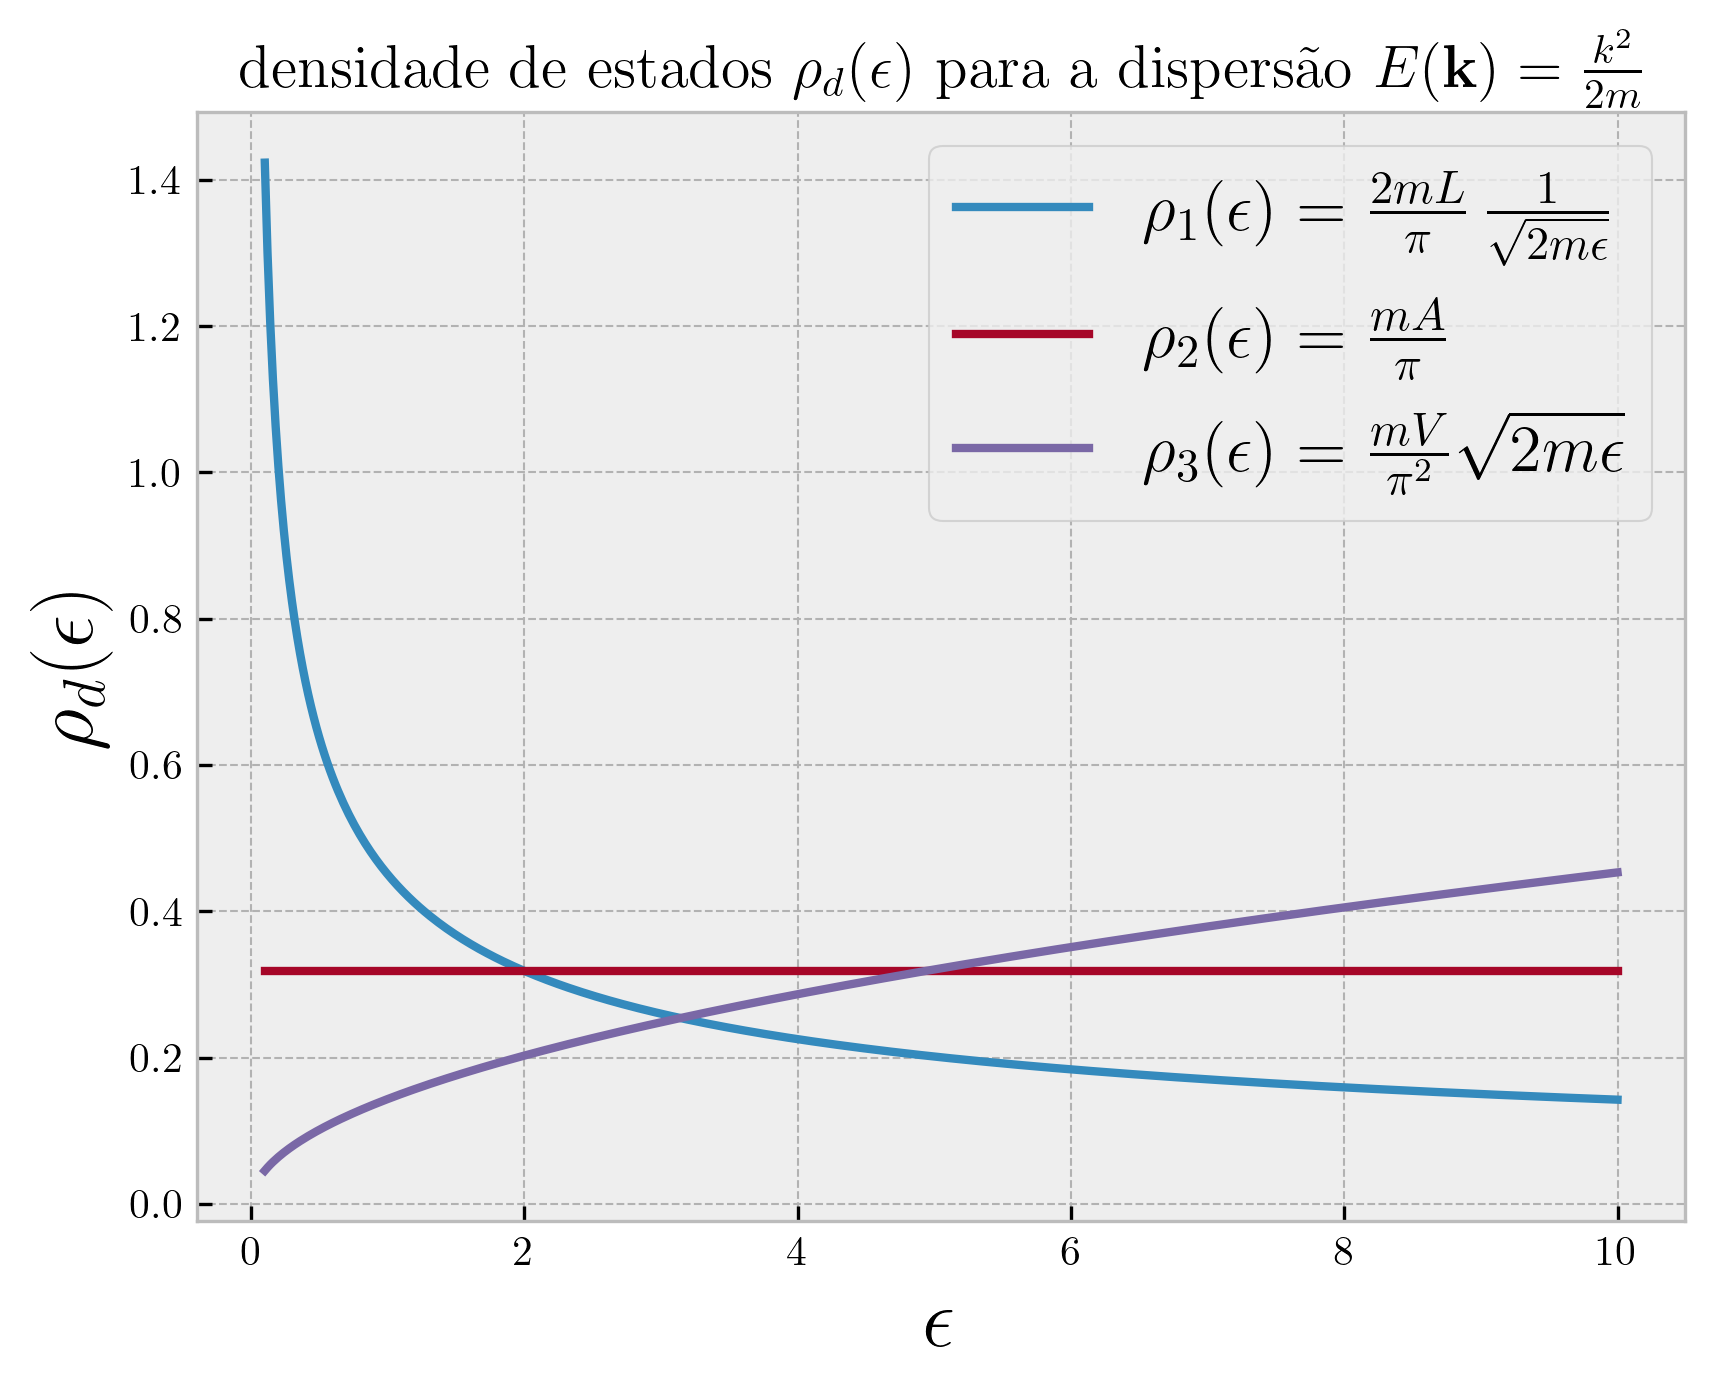
\includegraphics[width=0.5\textwidth]{fig/dos-k2.png}
\caption{Densidade de estados $\rho_d(\eps)$ para as dimensões $d = 1, 2$ e $3$. Parâmetros: $m = L = A = V = 1$.}
\label{fig:dosk2}
\end{figure}

(b) Analogamente para a dispersão $E(\k) = vk$:

%\url{https://eng.libretexts.org/Bookshelves/Materials_Science/Supplemental_Modules_(Materials_Science)/Electronic_Properties/Density_of_States}

$$
\rho_d(\eps) = \sum_{\k, \s} \delta(\eps - E(\k)) =
\frac{2V_d}{(2\pi)^d} \int \delta\qty(\eps - vk) \dd[d]{k} =
\frac{2V_d}{(2\pi)^d} \int \dd{\Omega_d} \int_0^\infty \delta\qty(\eps - vk) k^{d-1} \dd{k},
$$

Definindo dessa vez $g(k) = \eps - vk$, temos $\abs{g'(k)} = v$ e sua única raiz no domínio $D = (0, +\infty)$ é $k = \eps/v$. Portanto
$$
\rho_d(\eps) = \frac{2V_d}{(2\pi)^d} \Theta_d \, \frac{1}{v}
\qty(\frac{\eps}{v})^{d-1} = \frac{2 V_d \Theta_d}{(2\pi)^d v} \, \qty(\frac{\eps}{v})^{d-1}.
$$

Substituindo $d = 1, 2$ e $3$:
\begin{itemize}
\item $d = 1$, $V_1 = L$, $\Theta_1 = 2$:
$$
\rho_1(\eps) = \frac{2 L}{\pi v}.
$$
\item $d = 2$, $V_2 = A$, $\Theta_2 = 2\pi$:
$$
\rho_2(\eps) = \frac{A}{\pi v^2} \, \eps.
$$
\item $d = 3$, $V_3 = V$, $\Theta_3 = 4\pi$:
$$
\rho_3(\eps) = \frac{V}{\pi^2 v^3} \, \eps^2.
$$
\end{itemize}

\begin{figure}[H]
\centering
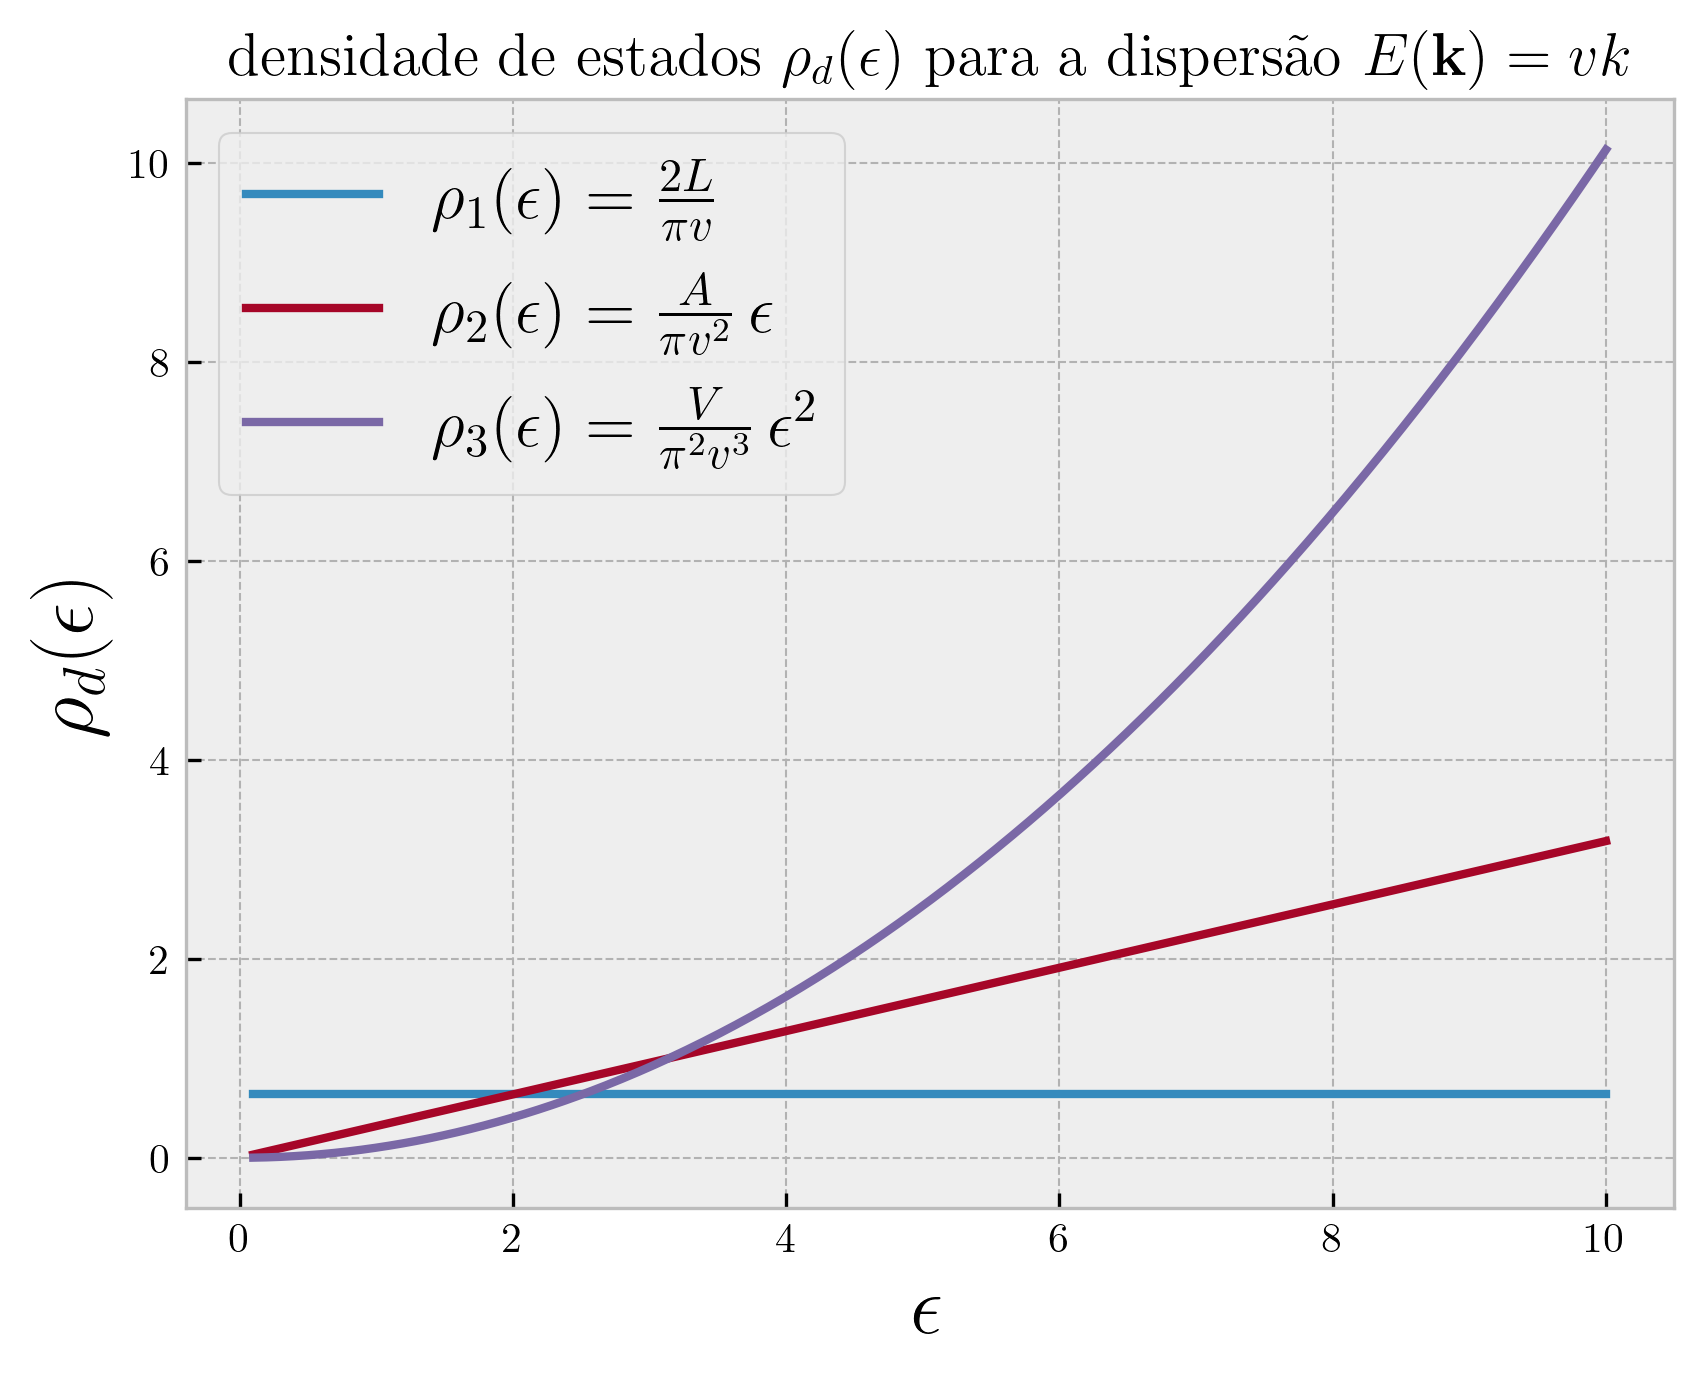
\includegraphics[width=0.5\textwidth]{fig/dos-vk.png}
\caption{Densidade de estados $\rho_d(\eps)$ para as dimensões $d = 1, 2$ e $3$. Parâmetros: $v = L = A = V = 1$.}
\label{fig:dosvk}
\end{figure}

\pagebreak

\section{Expansão de Sommerfeld}

(a) Façamos a substituição de variáveis $x = \beta(\eps - \mu)$, temos
$$
I = \frac{1}{\beta} \int_{-\infty}^{\infty} \frac{G(\mu + \frac{x}{\beta})}{e^{x} + 1} \dd{x}
$$
Já que $\displaystyle{\frac{1}{e^{-x} + 1} = \frac{e^x}{e^x + 1} = 1 - \frac{1}{e^x + 1}}$, a integral de $-\infty$ até $0$ se escreve como
$$
\int_{-\infty}^0 \frac{G(\mu + \frac{x}{\beta})}{e^{x} + 1} \dd{x} =
\int_0^{\infty} \frac{G(\mu - \frac{x}{\beta})}{e^{-x} + 1} \dd{x} =
\int_0^{\infty} G\qty(\mu - \frac{x}{\beta}) \dd{x} -
\int_0^{\infty} \frac{G(\mu - \frac{x}{\beta})}{e^{x} + 1} \dd{x}.
$$
Voltando à integral $I$, temos
$$
I =
\int_0^{\infty} G\qty(\mu - \frac{x}{\beta}) \frac{\dd{x}}{\beta} +
\frac{1}{\beta}
\int_0^{\infty}\frac{G(\mu + \frac{x}{\beta}) - G(\mu - \frac{x}{\beta})}{e^x + 1}\dd{x}
$$
A primeira integral acima se reescreve facilmente como
$$
\int_0^\infty G\qty(\mu - \frac{x}{\beta}) \frac{\dd{x}}{\beta} =
\int_{-\infty}^\mu G(\eps) \dd{\eps},
$$
enquanto que para $\beta \to \infty$
$$
G\qty(\mu + \frac{x}{\beta}) - G\qty(\mu - \frac{x}{\beta}) \approx \frac{2x}{\beta} G'(\mu),
$$
de maneira que
$$
\frac{1}{\beta}
\int_0^{\infty}\frac{G(\mu + \frac{x}{\beta}) - G(\mu - \frac{x}{\beta})}{e^x + 1}\dd{x}=
\frac{2 G'(\mu)}{\beta^2}
\int_0^{\infty}\frac{x}{e^x + 1}\dd{x} =
\frac{\pi^2}{6 \beta^2} \, G'(\mu).
$$

Portanto
$$
I = \int_{-\infty}^{\mu} G(\eps) \dd{\eps} + \frac{\pi^2}{6} T^2 \eval{\dv{G}{\eps}}_{\eps = \mu}.
$$

(b) Para $T \to 0$, temos que $\mu \approx \eps_F$ de maneira que
$$
n = \int_{-\infty}^{\infty} f(\eps) \rho(\eps) =
\int_{-\infty}^{\eps_F} \rho(\eps) \dd{\eps} +
\int_{\eps_F}^{\mu} \rho(\eps) \dd{\eps} +
\frac{\pi^2}{6} T^2 \rho'(\eps_F),
$$
onde aproximamos $\rho'(\mu) \approx \rho'(\eps_F)$. Temos ainda que
$$
\int_{-\infty}^{\eps_F} \rho(\eps) \dd{\eps} \approx n,
$$
$$
\int_{\eps_F}^{\mu} \rho(\eps) \dd{\eps} \approx \rho(\eps_F) \, (\mu - \eps_F).
$$

Portanto concluimos que
\begin{equation} \label{eq:chempot}
\mu \approx \eps_F - \frac{\pi^2}{6} T^2 \frac{\rho'(\eps_F)}{\rho(\eps_F)}.
\end{equation}

(c) Aproximando $\mu \approx \eps_F$ no limite $T \to 0$, temos
$$
E = \int_{-\infty}^{\infty} f(\eps) \eps \rho(\eps) \dd{\eps} \approx
\int_{-\infty}^{\eps_F} \eps \rho(\eps) \dd{\eps} +
(\mu - \eps_F) \eps_F \rho(\eps_F) +
\frac{\pi^2}{6} T^2 \eval{\dv{(\eps \rho(\eps))}{\eps}}_{\eps = \eps_F},
$$
onde aproximamos $\displaystyle{\int_{\eps_F}^{\mu} \eps \rho(\eps) \dd{\eps} \approx (\mu - \eps_F) \eps_F \rho(\eps_F)}$ e $\displaystyle{\eval{\dv{(\eps \rho(\eps))}{\eps}}_{\eps = \mu} \approx \eval{\dv{(\eps \rho(\eps))}{\eps}}_{\eps = \eps_F}}$.

\n

Substituindo então a aproximação \ref{eq:chempot} que obtivemos no item (b), obtemos
$$
E \approx \int_{-\infty}^{\eps_F} \eps \rho(\eps) \dd{\eps}
- \cancel{ \frac{\pi^2}{6} T^2 \eps_F \rho'(\eps_F) } +
\frac{\pi^2}{6} T^2 \Big[\rho(\eps_F) + \cancel{ \eps_F \rho'(\eps_F) } \Big],
$$
de maneira que
$$
c = \pdv{E}{T} \approx \frac{\pi^2}{3} T \rho(\eps_F).
$$


\pagebreak

\section{Susceptibilidade paramagnética do gás de elétrons}

(a) No limite $\mu_B h \to 0$, temos que $\mu$ não se altera significativamente, $\mu(h) \approx \mu(h = 0) = \mu$.

Metade dos elétrons tem spin up $+1/2$ e a outra metade tem spin down $-1/2$. Devido ao campo magnético, ocorre um splitting nas energias. Os elétrons de spin up ficam com uma energia $\eps \to \eps - \mu_B h$ e os de spin down com $\eps \to \eps + \mu_B h$. Com essas considerações, temos
$$
n_+ = \frac{1}{2} \int f(\eps) \rho(\eps - \mu_B h) \dd{\eps} \e
n_- = \frac{1}{2} \int f(\eps) \rho(\eps + \mu_B h) \dd{\eps},
$$
de maneira que $h = 0 \implies n_+ + n_- = \int f(\eps) \rho(\eps) \dd{\eps} = n$ (recuperamos o caso particular). A magnetização $m$ é dada por
$$
m = - \mu_B (n_+ - n_-) =
\frac{\mu_B}{2} \int f(\eps) \Big[ \rho(\eps + \mu_B h) - \rho(\eps - \mu_B h) \Big] \dd{\eps},
$$
mas como $\mu_B h \to 0$, temos $\rho(\eps + \mu_B h) - \rho(\eps - \mu_B h) \approx 2 \mu_B h \rho'(\eps)$. Integrando por partes:
\begin{equation} \label{eq:magnetization}
m = \mu_B^2 h \int_{-\infty}^{\infty} f(\eps) \rho'(\eps) \dd{\eps}
\end{equation}
$$
= \mu_B^2 h \qty(\eval{f(\eps) \rho(\eps)}_{-\infty}^{\infty} - \int \rho(\eps) f'(\eps) \dd{\eps} ).
$$
Mas $\rho(\pm\infty) = 0$, portanto
$$
m = \mu_B^2 h \int \rho(\eps) \qty(- \pdv{f}{\eps}) \dd{\eps} \implies
\chi = \pdv{m}{h} = \mu_B^2 \int \rho(\eps) \qty(- \pdv{f}{\eps}) \dd{\eps}.
$$

(b) Para $T = 0$, usando a equação \ref{eq:magnetization}, temos
$$
m = \mu_B^2 h \int_{-\infty}^{\infty} f(\eps) \rho'(\eps) \dd{\eps} =
\mu_B^2 h \int_{-\infty}^{\eps_F} \rho'(\eps) \dd{\eps} =
\mu_B^2 h \qty[ \rho(\eps_F) - \cancelto{0}{\rho(-\infty)} ]
$$
$$
\implies \chi = \mu_B^2 \rho(\eps_F).
$$

(c) Para $T \to \infty$ ($\beta \to 0$), aproximamos $f(\eps) \approx e^{-\beta(\eps - \mu)}$ de maneira que $\pdv{f}{\eps} = -\beta f(\eps)$. Portanto
$$
\chi(T \to \infty) = \mu_B^2 \int \rho(\eps) \qty(- \pdv{f}{\eps}) \dd{\eps} \approx
\mu_B^2 \beta \int f(\eps) \rho(\eps) \dd{\eps} = n \, \frac{\mu_B^2}{k_B T}.
$$


\pagebreak


\section{Teoria de perturbação para o gás de elétrons} \label{sec:pert}

(a) Em sala de aula vimos que a parte de Coulomb da hamiltoniana do Jellium se escreve como
\begin{equation} \label{eq:jellium}
\hat{V} = \frac{2 \pi e^2}{\mathcal{V}}
\sum_{\substack{\k_1, \k_2, \q \neq \0 \\ \s_1 \s_2}} \frac{1}{\q^2} \,
c_{\k_1 - \q, \s_1}^\d c_{\k_2 + \q, \s_2}^\d c_{\k_2 \s_2} c_{\k_1 \s_1}
\end{equation}

A correção de primeira ordem para a energia do ground-state é dada por
$$
E_0^{(1)} = \frac{\ev{\hat{V}}{\text{GS}}}{N},
$$
onde o ground-state do sistema é
$$
\ket{\text{GS}} = \prod_{\abs{\k} \leq k_{F}, \s} c_{\k \s}^{\d} \ket{0}.
$$

Assim, teremos que calcular
$$
M_{\k_1 \k_2 \q, \s_1 \s_2} = \ev{c_{\k_1 - \q, \s_1}^\d c_{\k_2 + \q, \s_2}^\d c_{\k_2 \s_2} c_{\k_1 \s_1}}{\text{GS}}.
$$

Para isso, podemos utilizar que $\ev{c_k^\d c_l^\d c_i c_j}{n_i n_j} = (\delta_{kj} \delta_{li} - \delta_{ki} \delta_{lj}) n_i n_j$ do item 2(e) da Lista 1, onde $k = (\k_1 - \q, \s_1)$; $l = (\k_2 + \q, \s_2)$; $i = (\k_2, \s_2)$ e $j = (\k_1, \s_1)$. Assim, obtemos que

$$
M_{\k_1 \k_2 \q, \s_1 \s_2} =
\Big(
\delta_{\k_1 - \q, \k_1} \delta_{\s_1, \s_1} \delta_{\k_2 + \q, \k_2} \delta_{\s_2, \s_2} -
\delta_{\k_1 - \q, \k_2} \delta_{\s_1, \s_2} \delta_{\k_2 + \q, \k_1} \delta_{\s_1, \s_2}
\Big) \ev{\nn_{\k_2 \s_2} \nn_{\k_1 \s_1}}{\text{GS}} =
$$
$$
=
\Big(
\delta_{\q, \0} -
\delta_{\q, \k_1 - \k_2} \delta_{\s_1, \s_2}
\Big) \ev{\nn_{\k_2 \s_2} \nn_{\k_1 \s_1}}{\text{GS}}.
$$

Como a equação \ref{eq:jellium} se trata de uma somatória com $\q \neq 0$, o termo $\delta_{\q, \0}$ vai desaparecer. Veja também que $\ev{\nn_{\k_2 \s_2} \nn_{\k_1 \s_1}}{\text{GS}} = \theta(k_F - \abs{\k_1}) \, \theta(k_F - \abs{\k_2})$, pois essa quantidade só é diferente de zero se ambos $\k_1$ e $\k_2$ estiverem dentro do mar de Fermi.

Assim
$$
\frac{\ev{\hat{V}}{\text{GS}}}{N} =
- \frac{2 \pi e^2}{N \mathcal{V}} \sum_{\substack{\k_1, \k_2, \q \neq \0 \\ \s_1 \s_2}}
\frac{1}{\q^2} \,
\delta_{\q, \k_1 - \k_2} \delta_{\s_1, \s_2} \theta(k_F - \abs{\k_1}) \, \theta(k_F - \abs{\k_2}).
$$
$$
= - \frac{2 \pi e^2}{N \mathcal{V}} \sum_{\s} \sum_{\q \neq \0} \frac{1}{\abs{\q}^2} \sum_{\k}
\theta(k_F - \abs{\k}) \, \theta(k_F - \abs{\k + \q}).
$$

A \textcolor{blue}{somatória nos spins $\sum_{\s}$ se converte em um fator $\bm{2}$} e as somatórias nos momentos nós convertemos em integrais via $\sum_{\k} \to \frac{\mathcal{V}}{(2\pi)^3} \int_{\R^3} \dd[3]{\k}$. Temos que
$$
I = \sum_{\q \neq \0} \frac{1}{\abs{\q}^2} \sum_{\k}
\theta(k_F - \abs{\k}) \, \theta(k_F - \abs{\k + \q}) =
\qty[ \frac{\mathcal{V}}{(2\pi)^3} ]^2 \int_{\R^3} \frac{\dd[3]{\q}}{\abs{\q}^2} \int_{\R^3}
\theta(k_F - \abs{\k}) \, \theta(k_F - \abs{\k + \q}) \dd[3]{\k}.
$$

Fixado $\q$, o termo de Heaviside $\theta(k_F - \abs{\k}) \, \theta(k_F - \abs{\k + \q})$ corresponde ao domínio de integração $D_{\q} = \{\k \in \R^3 \mid \abs{\k} < k_F\} \cap \{\k \in \R^3 \mid \abs{\k + \q} < k_F\}$, que é uma interseção de duas esferas com raio $k_F$, uma centrada em $\0$ e a outra em $-\q$. Note que esse domínio $D_{\q}$, não depende da direção de $\q$, somente do módulo $q$. Ainda mais, perceba que $D_q \neq \emptyset$ somente se $0 < q < 2 k_F$. Assim a integral $I$ se simplifica
$$
I = \qty[\frac{\mathcal{V}}{(2\pi)^3}]^2 \int_0^{2k_F} \frac{4\pi \, q^2 \dd{q}}{q^2} \int_{D_q} \dd[3]{\k} =
\qty[\frac{\mathcal{V}}{(2\pi)^3}]^2 (4\pi) \int_0^{2k_F} \text{Vol}(D_q) \dd{q}.
$$
Assim, precisamos calcular $\text{Vol}(D_q) = \int_{D_q} \dd[3]{\k}$, que é o volume da interseção das duas esferas. Se fizermos o desenho geométrico (não vou fazer aqui pois dá trabalho, mas o Bruus-Flensberg faz esse cálculo na página 42) e utilizarmos coordenadas polares $(k, \theta_k, \vphi_k)$ é fácil ver que
$$
\text{Vol}(D_q) = 2 \int_0^{2\pi} \dd{\vphi_k} \int_{q / (2 k_F)}^{1} \dd(\cos\theta_k) \int_{q / (2 \cos\theta_k)}^{k_F} k^2 \dd{k} = \frac{4\pi}{3} k_F^3 - \pi k_F^2 q + \frac{\pi}{12} q^3.
$$

E portanto
$$
I = \qty[\frac{\mathcal{V}}{(2\pi)^3}]^2 (4\pi) \, (\pi k_F^4) \implies
E_0^{(1)} = - \frac{2 \pi e^2}{N \mathcal{V}} \times 2 \times
\qty[\frac{\mathcal{V}}{(2\pi)^3}]^2 (4\pi) \, (\pi k_F^4)
= - e^2 \frac{\mathcal{V}}{N}
\frac{16 \pi^3 }{(2\pi)^6} k_F^4 .
$$

Finalmente, usando que $n = \frac{N}{\mathcal{V}}$ e $\displaystyle{ k_F = \sqrt[3]{3 \pi^2 n} = \frac{1}{a_0 r_s} \qty(\frac{9\pi}{4})^{1/3} }$, obtemos
\begin{equation} \label{eq:1ord}
E_0^{(1)} =
- e^2 \cdot \frac{k_F^3}{n} \cdot
\frac{1}{4 \pi^3} \cdot k_F
\end{equation}
$$
= - e^2 \cdot \frac{3}{4 \pi} \cdot \frac{1}{a_0 r_s} \qty(\frac{9\pi}{4})^{1/3}
= - \frac{3}{2\pi} \qty(\frac{9\pi}{4})^{1/3} \frac{1}{r_s} \, \qty(\frac{e^2}{2a_0}) \implies
$$
$$
E_0^{(1)}
= - \frac{3}{2\pi} \qty(\frac{9\pi}{4})^{1/3} \frac{1}{r_s} \, \text{Ry}.
$$

\n

(b) Numa célula esférica uniformemente carregada com densidade $+ne$, um elétron localizado num raio $r$ enxerga a força de Coulomb somente da bola positiva de raio $r$, como se toda carga dessa bola estivesse no centro. Assim, a força que o elétron sente é
$$
F(\r) = -\grad{V} = - \frac{e^2}{r^2} n(r) \vu{r} = -\frac{e^2}{a_0^3 r_s^3} r \, \vu{r},
$$
onde $n(r) = n \frac{4 \pi}{3} r^3 = \qty(\frac{r}{a_0 r_s})^3$. Portanto, o potencial que o elétron sente é
$$
V(\r) = \frac{1}{2} \, \frac{e^2}{a_0^3 r_s^3} r^2,
$$
que é um potencial harmônico tridimensional. Escrevemos $V(\r) = \frac{1}{2} m \omega_0^2 \r^2$, com $\omega_0^2 = \frac{e^2}{m a_0^3 r_s^3}$. Lembrando que $a_0 = \frac{1}{m e^2}$ ($\hbar = 1$), a energia de ponto zero corresponde à energia $\frac{3}{2} \omega_0$ do estado fundamental do oscilador harmônico tridimensional:
$$
\frac{E_{\text{Wigner}}^{(1)}}{N} = \frac{3}{2} \omega_0 =
\frac{3}{2} \, \frac{e}{\sqrt{m a_0^3}} \, \frac{1}{r_s^{3/2}} =
\frac{3 e^2}{2 a_0} \, \frac{1}{r_s^{3/2}} = \frac{3}{r_s^{3/2}} \, \text{Ry}.
$$


\pagebreak

\section{Gás de elétrons polarizado}

(a) Sejam $k_{F \up}$ e $k_{F \down}$ os números de Fermi para spin $\up$ e $\down$. Temos
$$
N_{\up} = \sum_{\k} \ev{n_{\k \up}}{\text{GS}} =
\frac{\mathcal{V}}{(2\pi)^3} \int \dd[3]{\k} \theta(k_{F\up} - k) = \frac{V}{6 \pi^2} k_{F\up}^3 \implies
k_{F\up} = \sqrt[3]{3 \pi^2 n (1 + \xi)},
$$
analogamente para $k_{F\down} = \sqrt[3]{3 \pi^2 n (1 - \xi)}$. Para o termo de energia cinética temos
$$
\frac{E_{\text{pol}}^{(0)}}{N} = \frac{1}{N} \sum_{\k \s} \frac{\hbar^2 k^2}{2m} \ev{n_{\k\s}}{\text{GS}} =
\frac{V}{(2 \pi)^3 N} \, \frac{\hbar^2}{2m} \int \dd[3]{\k} \qty[ \theta(k_{F\up} - k) + \theta(k_{F\down} - k) ] =
$$
$$
= \frac{V}{(2 \pi)^3 N} \, \frac{\hbar^2}{2m} \, 4 \pi \qty[\int_0^{k_{F\up}} k^4 \dd{k} + \int_0^{k_{F\down}} k^4 \dd{k}]
= \frac{1}{10 \pi^2 n} \, \frac{\hbar^2}{2m} \qty(k_{F\up}^5 + k_{F\down}^5).
$$

Substituindo $k_{F\up\down} = \sqrt[3]{3 \pi^2 n (1 \pm \xi)}$, $n = \frac{3}{4\pi (r_s a_0)^3}$, $a_0 = \frac{\hbar^2}{m e^2}$ e $\text{Ry} = \frac{e^2}{2a_0}$, obtemos
$$
\frac{E_{\text{pol}}^{(0)}}{N} = \frac{3}{10} \qty(\frac{9\pi}{4})^{2/3} \frac{1}{r_s^2}
\qty[(1+\xi)^{5/3} + (1-\xi)^{5/3}] \, \text{Ry}.
$$

(b) Para a correção de primeira ordem do gás polarizado, os cálculos são análogos à Questão \ref{sec:pert}. Podemos usar diretamente o resultado da equação \ref{eq:1ord}, dividindo o resultado por $2$ (porque o spin não é simétrico mais) e separando $k_{F\up}$ e $k_{F\down}$:
$$
\frac{E_{\text{pol}}^{(1)}}{N} =
- \frac{e^2}{2} \, \frac{1}{4\pi^3} \qty(\frac{k_{F\up}^3}{n} \, k_{F\up} + \frac{k_{F\down}^3}{n} \, k_{F\down}) =
\frac{-3e^2}{2 \cdot 4\pi} n^{1/3} \qty[(1+\xi)^{4/3} + (1-\xi)^{4/3}] \implies
$$
$$
\frac{E_{\text{pol}}^{(1)}}{N} =
- \frac{3}{4\pi} \qty(\frac{9\pi}{4})^{1/3} \frac{1}{r_s} \, \qty[(1+\xi)^{4/3} + (1-\xi)^{4/3}] \, \text{Ry}.
$$

Defina $\Sigma(\xi) = \frac{E_{\text{pol}}^{(0)} + E_{\text{pol}}^{(1)}}{N}$ como a energia do estado fundamental como função da polarização $\xi$:
$$
\Sigma(\xi) =
\frac{1}{2} \qty{ \frac{3}{5} \qty(\frac{9\pi}{4})^{2/3} \frac{1}{r_s^2}
\qty[(1+\xi)^{5/3} + (1-\xi)^{5/3}]
- \frac{3}{2\pi} \qty(\frac{9\pi}{4})^{1/3} \frac{1}{r_s} \qty[(1+\xi)^{4/3} + (1-\xi)^{4/3}]
} \, \text{Ry}.
$$

Então analizamos os valores de $r_s$ para quais $\Sigma(\xi = 1) < \Sigma(\xi = 0)$. Isso nos dá que
$$
\Sigma(1) < \Sigma(0) \implies
$$
$$
\frac{3}{5} \qty(\frac{9\pi}{4})^{2/3} \frac{2^{2/3}}{r_s^2}
- \frac{3}{2\pi} \qty(\frac{9\pi}{4})^{1/3} \frac{2^{1/3}}{r_s} \; < \;
\frac{3}{5} \qty(\frac{9\pi}{4})^{2/3} \frac{1}{r_s^2}
- \frac{3}{2\pi} \qty(\frac{9\pi}{4})^{1/3} \frac{1}{r_s} \implies
$$
$$
\frac{2\pi}{5} \qty(\frac{9\pi}{4})^{1/3} 2^{2/3} - 2^{1/3} r_s \; < \;
\frac{2\pi}{5} \qty(\frac{9\pi}{4})^{1/3} - r_s \implies
$$
$$
(2^{1/3} - 1) \, r_s \; > \; \frac{2\pi}{5} \qty(\frac{9\pi}{4})^{1/3} (2^{2/3} - 1)
$$
$$
r_s \; > \; \qty(\frac{2\pi}{5}) \qty(\frac{9\pi}{4})^{1/3} (2^{1/3} + 1) = 5.45.
$$

O resultado acima indica que, para valores de $r_s$ altos o suficiente (a saber da ordem de $5.45$), o estado fundamental do sistema é \textbf{ferromagnético}, já que a energia desse estado é menor do que a energia do estado não-polarizado.



\pagebreak

\end{document}
